% Chapter 1

\chapter{Results} % Main chapter title

\label{Chapter3} % For referencing the chapter elsewhere, use \ref{Chapter1} 

\lhead{Chapter 3. \emph{Results}} % This is for the header on each page - perhaps a shortened title

%----------------------------------------------------------------------------------------
\begin{comment}
Order of Presentation
Offer your results in an order that is similar to the order you presented your
hypothesis or research questions.

Descriptive Data
Provide all the descriptive data such as demographic results.

Results of Statistical Testing
Give the results of the statistical processes conducted for your study. Provide
only the results and avoid offering conclusions or interpretations of the results.

Interpretations of Statistical Results
Offer a brief summary of the results with foundational interpretations of what the
statistics provide.






This chapter presents the evidence and/or results of primary research which
you have undertaken. 
Depending upon your subject area this can be in the form
of detailed quantitative models, hypothesis testing to some basic analysis using
basic descriptive statistics or qualitative techniques dealing with structured
content analysis, textual analysis, to case study descriptions.
The main part of the chapter is the presentation of the data that you obtained.
Even projects of relatively moderate dimensions will generate a large amount
of data which has to be considered. 
This data must be organised in a logical
and coherently ordered whole so that your thought processes and
interpretation are clear to the reader.
Whatever form of data analysis has been undertaken, it must be accomplished
with care and attention to detail, as should the way in which the results are
presented. 
Nothing is guaranteed to frustrate a reader more than to have to
plough their way through an arid mass of tables, figures and statistics. Better by
far to describe in an accessible manner (which does not mean that you should
talk down to the reader) what the research has uncovered and to include only
the most pertinent figures as evidence of your findings. 
Dissertations which
included detailed modelling or quantitative analysis will clearly need to show
all relevant assumptions, relationships and methods. Your academic supervisor
will be able to advise on the level of detail required in the main body as
opposed to that included in the Appendix.
Graphs, diagrams, pie-charts etc. are all useful ways of presenting research
results; they are an imaginative way of ‘breaking up’ solid blocks of text – they
let a little ‘light’ into the body of the text as long as they are relevant and
illustrate your points. 
Keep your review to those items which are relevant to
your research question and not just everything I found out.
There will be problems in the execution of any research project and their
occurrence should be brought to the attention of the reader. 
Without stating
them, one of the essential elements of the context in which the research took
place will be missing.
Not all dissertations contain quantitative data. In many situations, students will
have made extensive use of qualitative research techniques such as focus
groups and/or in-depth unstructured interviews. 
While quantitative data lends
itself to graphs, tables and so on, qualitative data, and the way it is presented,
12
pose particular challenges for students. 
As ever, your objective should be based
on the belief that the data must be presented in such a manner as to make it
easy for the reader to follow the logic of the analysis.
The analysis of qualitative data should be based on the research questions and
issues that you explored during your fieldwork. 
For instance, you may have
addressed six or seven critical questions in a series of interviews. 
Each of these
questions should be examined separately, rather than describing each focus
group in turn. This provides a degree of logical flow and development to the
analysis. 
In addition, it is advisable to focus on the points of agreement and
disagreement that emerged during the interviews. 
This should be supported
with relevant quotations from the transcripts of the interviews. You should
avoid lengthy quotations, unless they are of critical importance. 
However, short
excerpts enrich the reader’s understanding of the issues and provide you with
the opportunity to shed a clearer insight on the topic.
Many students make the mistake of providing a very superficial, descriptive
analysis of qualitative data. 
This does not allow you to demonstrate that the
research you undertook was of a substantive nature. 
Tables can also be
included that reflect the respondent’s overall attitudes, perceptions and views
about the themes.
You are not required to include all the transcripts of interviews, surveys or data
sheets. 
Only include the summarised data in the main body of the dissertation.

Appendixes should be restricted to no more than 25 pages. 
You can keep additional information in a folder for use by the markers if requested.
In the case of company projects you may need to include some brief outline about the company and its activities. 
Again keep these comments focused on the topic area and not just a broad and general description of everything you know about the organisation.




\end{comment}

\section{SDSS Data}

matrix plot of examples
% \begin{figure}[htbp]
%   \centering
%     \includegraphics{./Figures/file_name}
%     \rule{35em}{0.5pt}
%   \caption[title]{caption.}
%   \label{fig:}
% \end{figure}

% Class_Moving Object0_rescaled_diff_img.jpg
% Class_Other SN3_rescaled_diff_img.jpg
% Class_Saturated Star0_rescaled_diff_img.jpg
% Class_Silver SN1_rescaled_diff_img.jpg
% Class_Transient4_rescaled_diff_img.jpg
% Class_Variable1_rescaled_diff_img.jpg
% Class_Artifact4_rescaled_diff_img.jpg
% Class_Bronze SN2_rescaled_diff_img.jpg
% Class_Dipole2_rescaled_diff_img.jpg
% Class_Gold SN2_rescaled_diff_img.jpg




TSNE Plots

\begin{figure}[htbp]
  \centering
    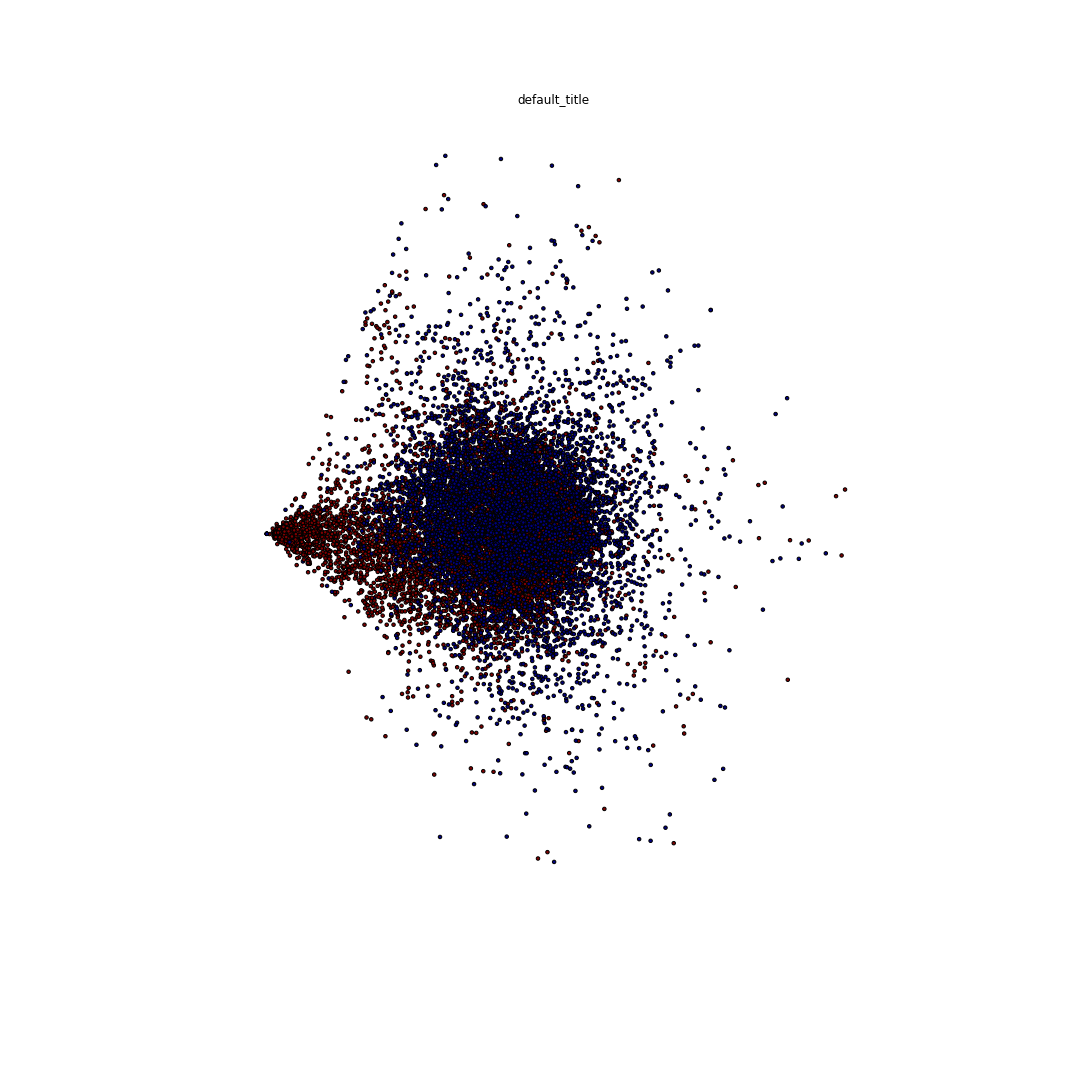
\includegraphics[width = 0.8\textwidth]{./Figures/binary_perp0.png}
    \rule{35em}{0.5pt}
  \caption[Binary TSNE]{caption.}
  \label{fig:}
\end{figure}

\begin{figure}[htbp]
  \centering
    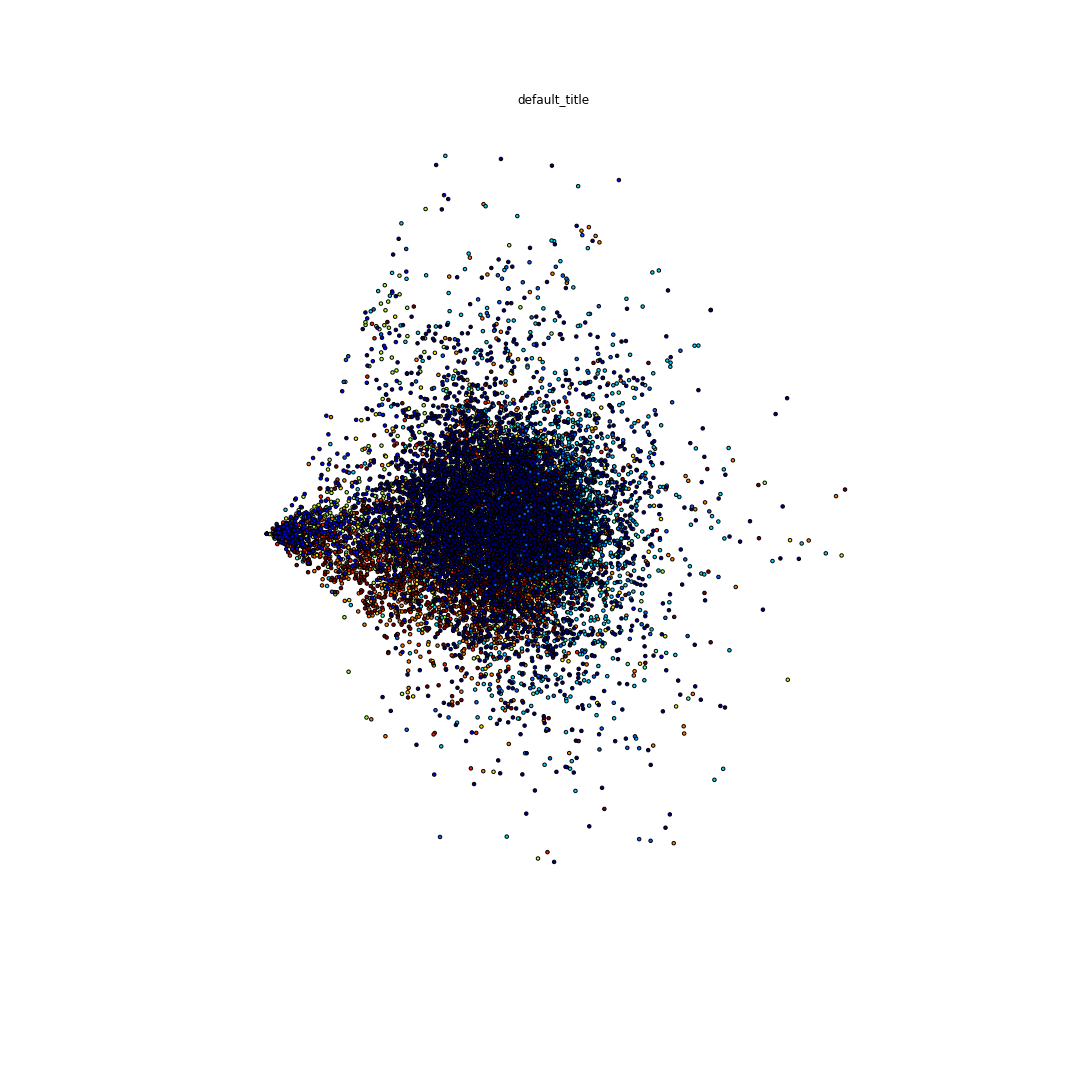
\includegraphics[width = 0.8\textwidth]{./Figures/10Classes_perp0.png}
    \rule{35em}{0.5pt}
  \caption[Multi-class TSNE]{caption.}
  \label{fig:}
\end{figure}



\section{Training Tricks}

Data Augmentation
	Translation
    Rotation
    
    


    \begin{figure}[htbp]
  \centering
    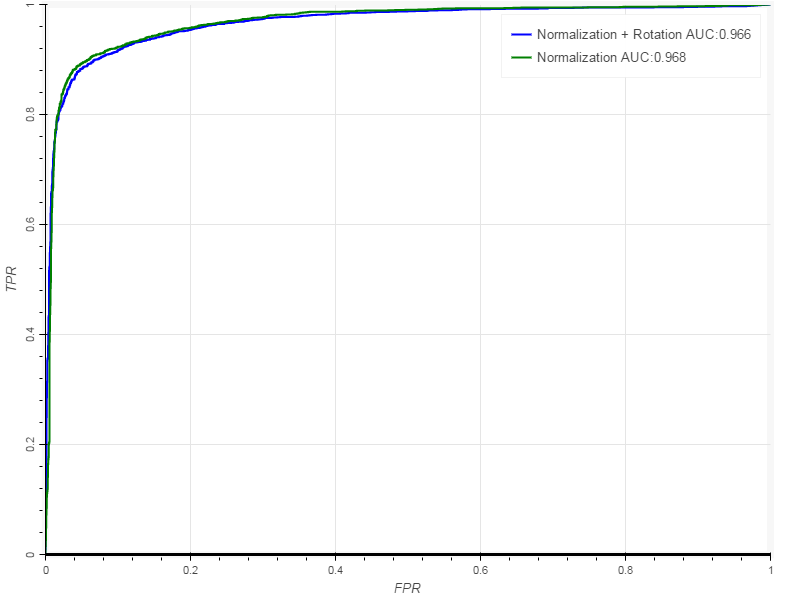
\includegraphics[width = 0.8\textwidth]{./Figures/AUC_rotation_mdl0.png}
    \rule{35em}{0.5pt}
  \caption[Rotation Augmentation]{caption.}
  \label{fig:}
\end{figure}

    Normalization
    
\begin{figure}[htbp]
  \centering
    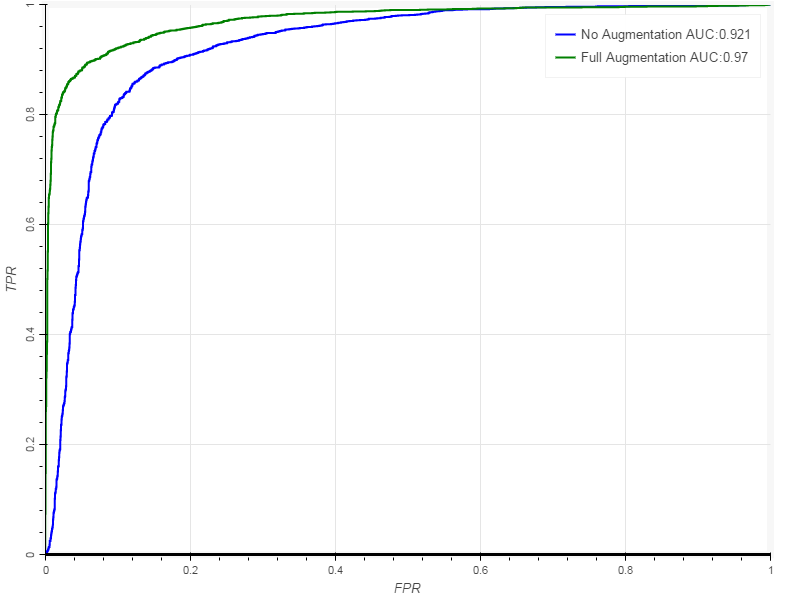
\includegraphics[width = 0.8\textwidth]{./Figures/AUC_augmentation_mdl0.png}
    \rule{35em}{0.5pt}
  \caption[Some vs. None Augmentation]{caption.}
  \label{fig:}
\end{figure}



CNN Model Designs

Model Selection

\section{Hyper-parameter Optimization}

  Batch Size

  Search and/or difference images
  
\begin{figure}[htbp]
  \centering
    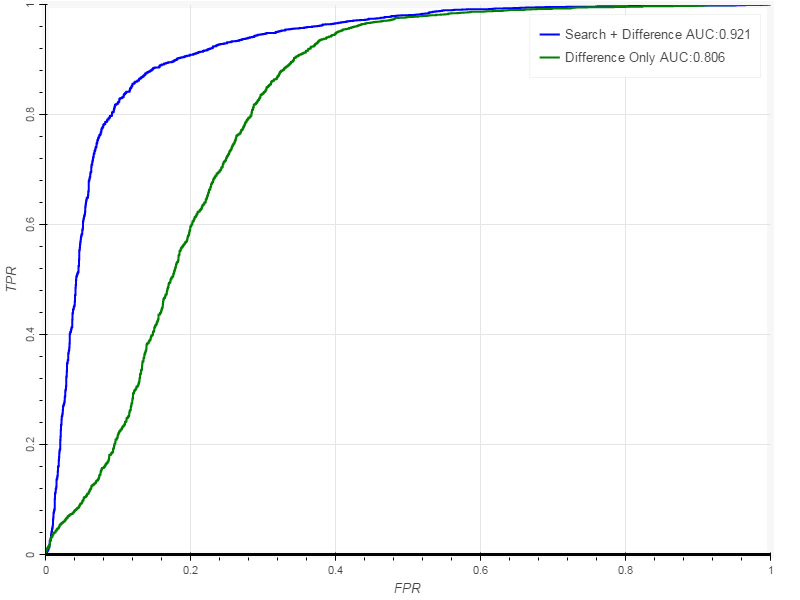
\includegraphics[width = 0.8\textwidth]{./Figures/AUC_search_mse.png}
    \rule{35em}{0.5pt}
  \caption[Search and/or Difference Images]{caption.}
  \label{fig:}
\end{figure}


  Batch Normalization
  
\begin{figure}[htbp]
  \centering
    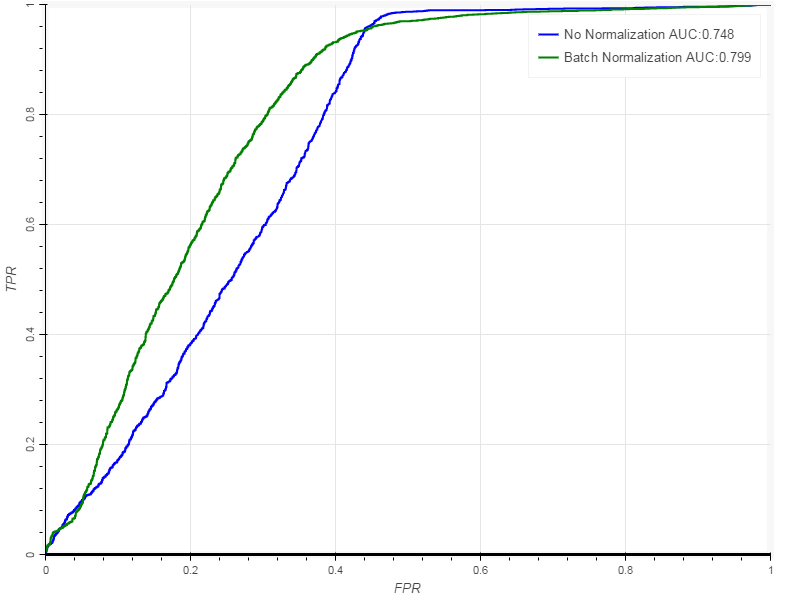
\includegraphics[width = 0.8\textwidth]{./Figures/AUC_batchnorm.png}
    \rule{35em}{0.5pt}
  \caption[Batch Normalization]{caption.}
  \label{fig:}
\end{figure}


  Drop-out
  
\begin{figure}[htbp]
  \centering
    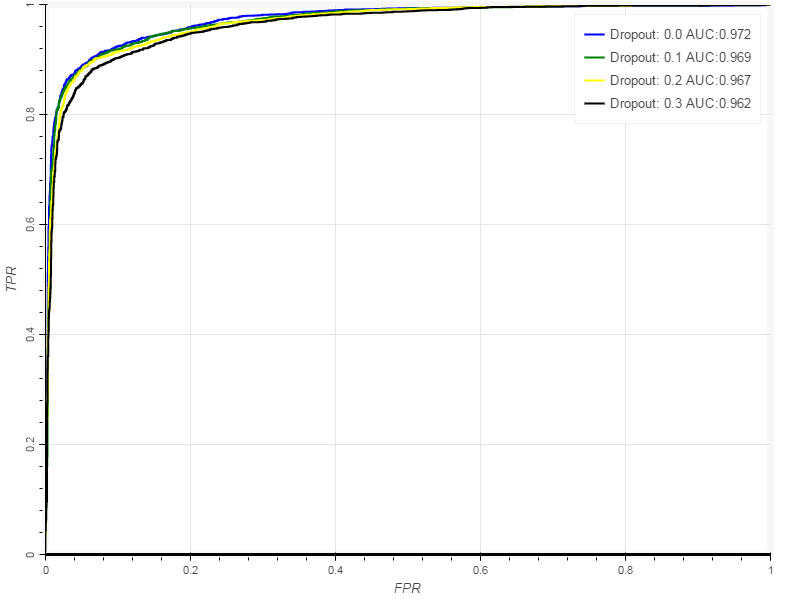
\includegraphics[width = 0.8\textwidth]{./Figures/AUC_dropout_mdl0.png}
    \rule{35em}{0.5pt}
  \caption[Dropout Performance]{caption.}
  \label{fig:}
\end{figure}

\begin{figure}[htbp]
  \centering
    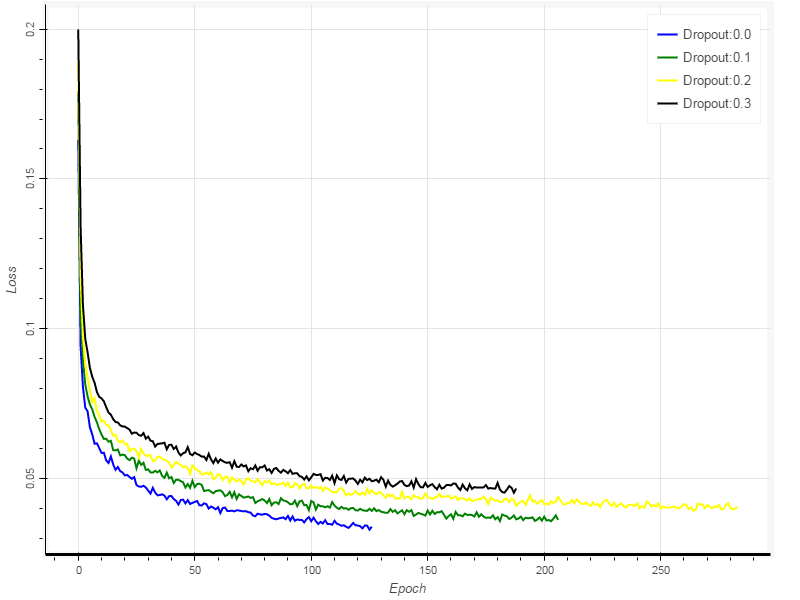
\includegraphics[width = 0.8\textwidth]{./Figures/training_dropout_mdl0.png}
    \rule{35em}{0.5pt}
  \caption[Dropout Training]{caption.}
  \label{fig:}
\end{figure}


  Regularization
  
\begin{figure}[htbp]
  \centering
    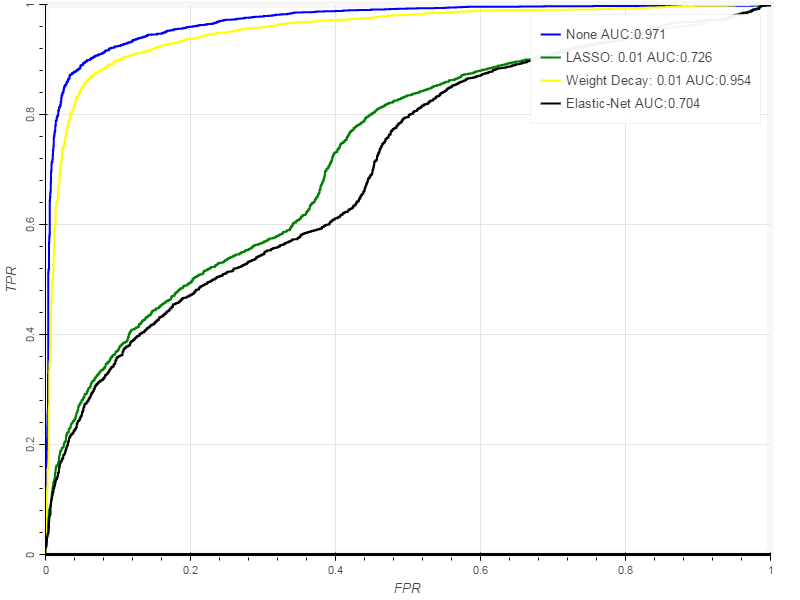
\includegraphics[width = 0.8\textwidth]{./Figures/AUC_regularization_mdl0.png}
    \rule{35em}{0.5pt}
  \caption[Regularization]{caption.}
  \label{fig:}
\end{figure}


  Network Activation Function
  
\begin{figure}[htbp]
  \centering
    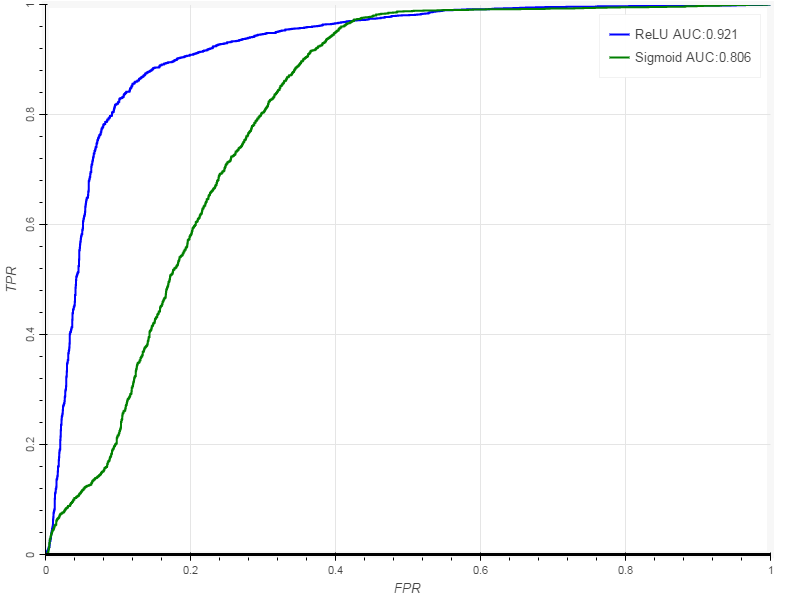
\includegraphics[width = 0.8\textwidth]{./Figures/AUC_activations.png}
    \rule{35em}{0.5pt}
  \caption[Activations]{caption.}
  \label{fig:}
\end{figure}


  Filter Size
\begin{figure}[htbp]
  \centering
    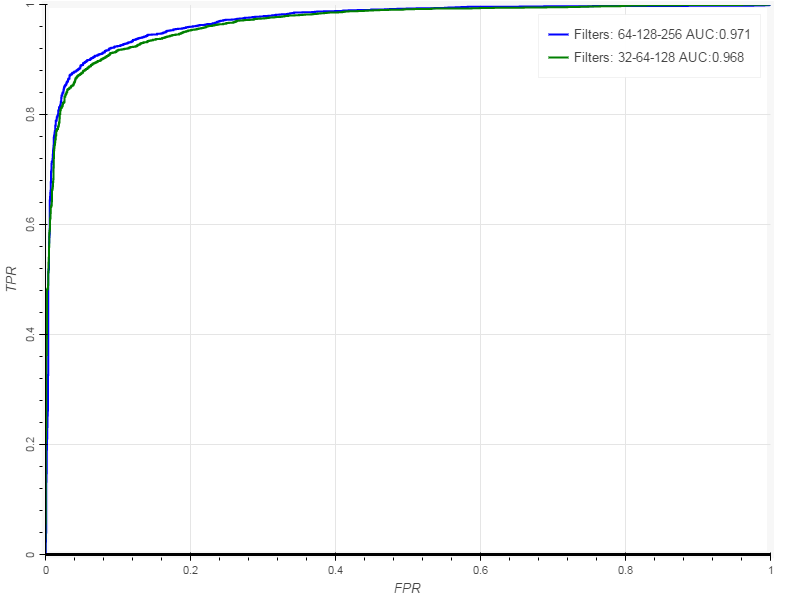
\includegraphics[width = 0.8\textwidth]{./Figures/AUC_filters_mdl0.png}
    \rule{35em}{0.5pt}
  \caption[Filter Size Performance]{caption.}
  \label{fig:}
\end{figure}

\begin{figure}[htbp]
  \centering
    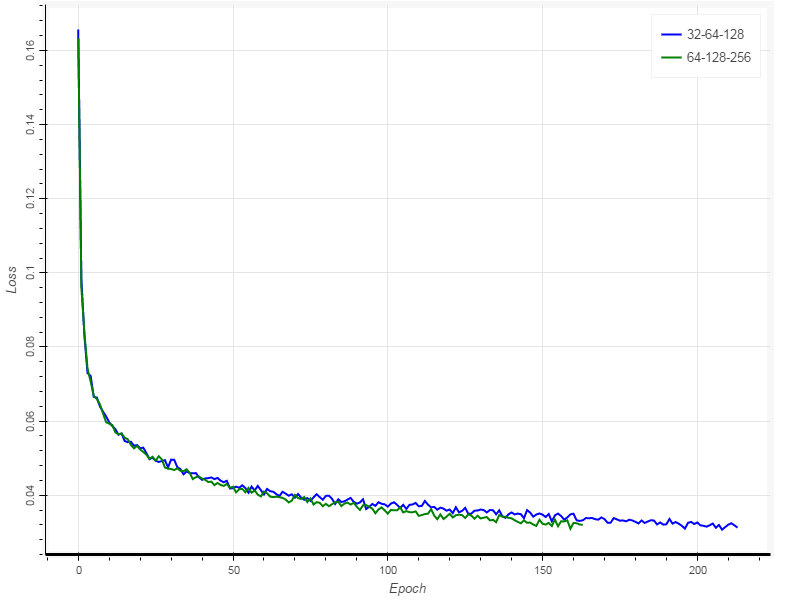
\includegraphics[width = 0.8\textwidth]{./Figures/training_filter_size_mdl0.png}
    \rule{35em}{0.5pt}
  \caption[Filter Size Training]{caption.}
  \label{fig:}
\end{figure}

  Update Algorithm

  Loss Function
\begin{figure}[htbp]
  \centering
    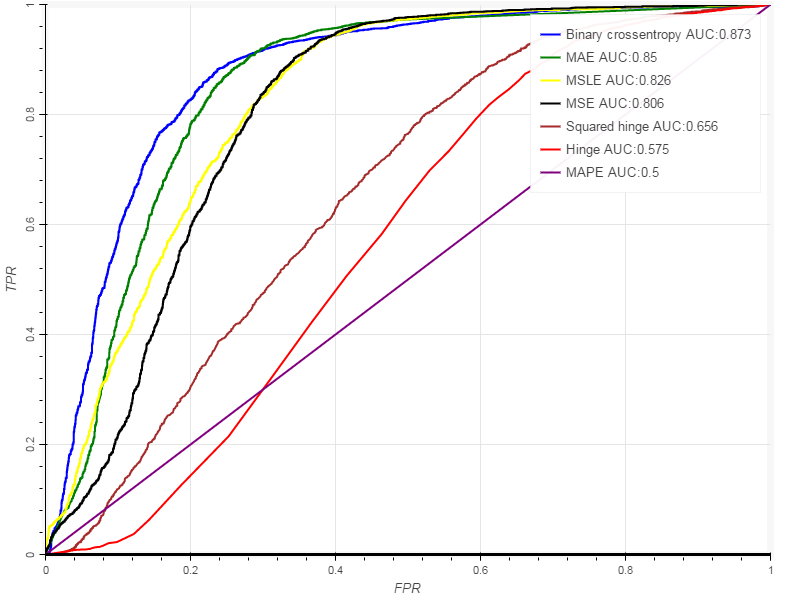
\includegraphics[width = 0.8\textwidth]{./Figures/AUC_loss_functions.png}
    \rule{35em}{0.5pt}
  \caption[Loss Functions]{caption.}
  \label{fig:}
\end{figure}


  number of neurons in final layers
\begin{figure}[htbp]
  \centering
    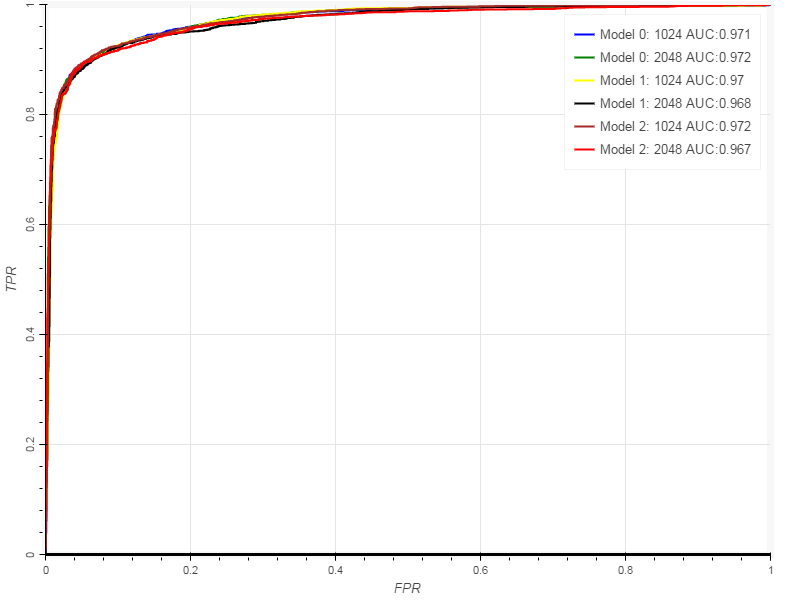
\includegraphics[width = 0.8\textwidth]{./Figures/AUC_final_neurons.png}
    \rule{35em}{0.5pt}
  \caption[Last Hidden Layers]{caption.}
  \label{fig:}
\end{figure}


BEST MODELS
\begin{figure}[htbp]
  \centering
    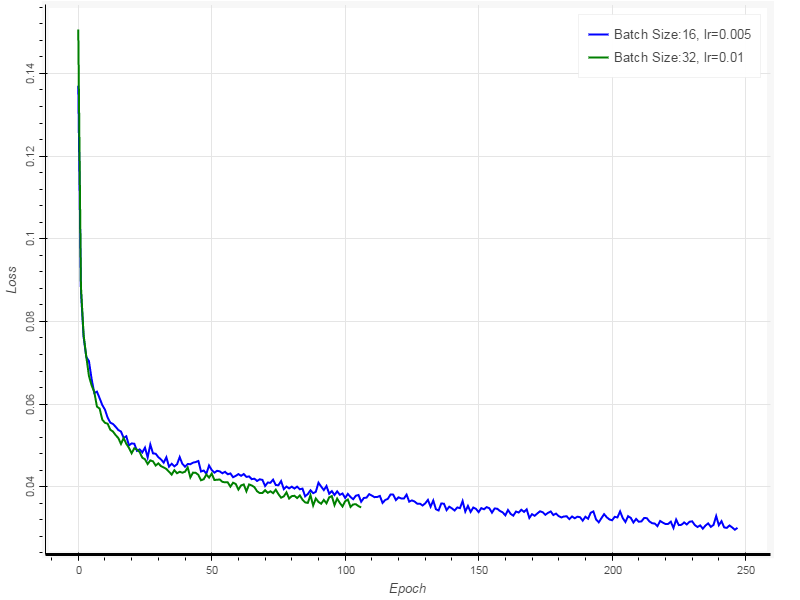
\includegraphics[width = 0.8\textwidth]{./Figures/training_slow_mdl0.png}
    \rule{35em}{0.5pt}
  \caption[Slow Training]{caption.}
  \label{fig:}
\end{figure}

\begin{figure}[htbp]
  \centering
    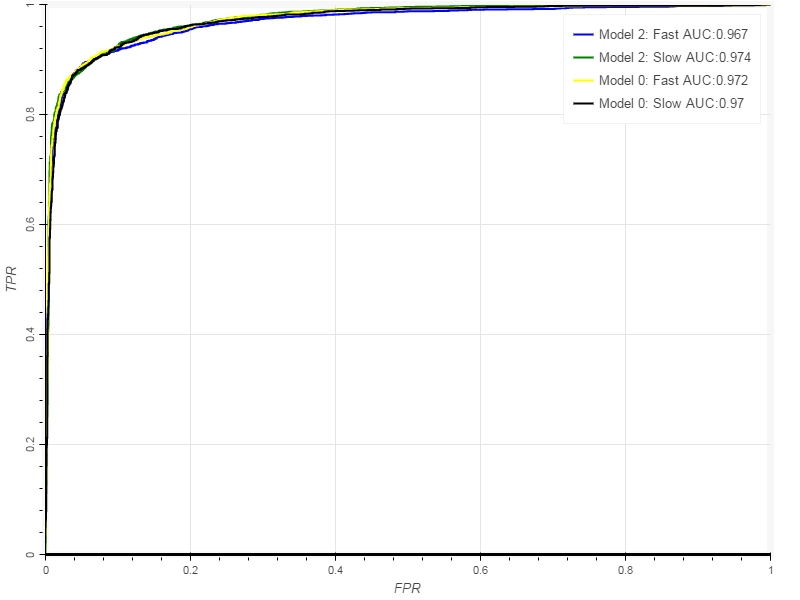
\includegraphics[width = 0.8\textwidth]{./Figures/AUC_best_models.png}
    \rule{35em}{0.5pt}
  \caption[Slow Training Performance]{caption.}
  \label{fig:}
\end{figure}

\section{Model Analysis}

  TSNE of final layer of activation
  
  Layer Kernel Visualization

  Confusion Matrices



% \subsection{Multi-class Classification}

%   AUC Score
  
%   Confusion Matrices

%   Multi-Class to Binary performance

%   TSNE at final layer of activation
  
\section{Comparative Performance}

  AUC Score

  Fake SNe

  Confirmed SNE
  
  miss-classified examples
